\documentclass[arhiv]{../izpit}
\usepackage{fouriernc}
\usepackage{xcolor}
\usepackage{tikz}

\begin{document}

\izpit{Programiranje I: 2.\ izpit}{19.\ februar 2016}{
  Čas reševanja je 120 minut.
  \textbf{Funkcij ne pozabite opremiti z ustrezno signaturo.}
  Veliko uspeha!
}

%%%%%%%%%%%%%%%%%%%%%%%%%%%%%%%%%%%%%%%%%%%%%%%%%%%%%%%%%%%%%%%%%%%%%%
\naloga[Kopice, 40 točk]

Drevesa s poljubnim številom sinov in vrednostmi v vozliščih lahko v Haskellu predstavimo
s podatkovnim tipom:
\begin{verbatim}
data Drevo a = Drevo a [Drevo a]
\end{verbatim}
Na primer, drevo
\[
  \begin{tikzpicture}
    \node (d) {18}
      child {node {12}}
      child {node {10}
        child {node {5}}
      }
      child {node {8}
        child {node {1}}
        child {node {3}}
      }
    ;
  \end{tikzpicture}
\]
bi predstavili kot
\begin{verbatim}
Drevo 18 [
  Drevo 12 [],
  Drevo 10 [Drevo 5 []],
  Drevo 8 [Drevo 1 [], Drevo 3 []]
]
\end{verbatim}

\noindent
Za takšno drevo pravimo, da je \emph{kopica}, če je vrednost korena večja od vseh
vrednosti korenov sinov, ti pa so prav tako kopice. Na primer, zgornje
drevo je kopica, spodnje pa ne, ker je vrednost 9 večja od 8.
  \[
    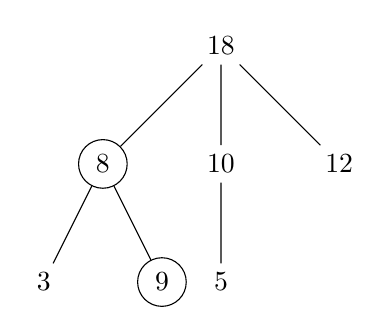
\begin{tikzpicture}
      \node (e) {18}
        child {node[draw, circle] {8}
          child {node {3}}
          child {node[draw, circle] {9}}
        }
        child {node {10}
          child {node {5}}
        }
        child {node {12}}
      ;
    \end{tikzpicture}  
  \]

\podnaloga[10 točk]
  Sestavite funkcijo \verb|vsota|, ki vrne vsoto vseh elementov v drevesu.
  Na primer, za prvo drevo bi funkcija vrnila $57$, za drugo pa $65$.

\podnaloga[10 točk]
  Sestavite funkcijo \verb|jeKopica|, ki vrne \verb|True|, če je dano drevo
  kopica, in \verb|False| sicer.

\podnaloga[10 točk]
  Sestavite funkcijo
\begin{verbatim}odstraniMax :: Ord a => Drevo a -> (a, Maybe (Drevo a))
\end{verbatim}
 ki vrne največji element dane kopice ter kakršnokoli
  kopico, ki vsebuje vse preostale sinove. Če iz drevesa odstranimo
  zadnji element, naj bo druga komponenta vrnjenega para enaka \verb|Nothing|.

\podnaloga[10 točk]
  S pomočjo prejšnje funkcije napišite funkcijo \verb|padajociElementi|, ki
  vrne seznam vseh elementov kopice, urejen od največjega proti najmanjšemu.


%%%%%%%%%%%%%%%%%%%%%%%%%%%%%%%%%%%%%%%%%%%%%%%%%%%%%%%%%%%%%%%%%%%%%%
\naloga[Zlaganje kock, 20 točk]

Nalogo lahko rešujete v Haskellu ali v Pythonu.
 
\podnaloga[10 točk + 5 točk] Na voljo imamo poljubno število kock velikosti $1 \times 1 \times 1$, $2 \times 2 \times 2$
  in $3 \times 3 \times 3$. Na koliko različnih načinov lahko sestavimo stolp višine $n$?
  Pri tem lahko postavimo tudi večjo kocko na manjšo. Kock istih velikosti ne ločimo med seboj. 
  Sestavite funkcijo, ki izračuna število vseh različnih stolpov višine $n$, ki jih
  lahko sestavimo iz danih kock. Na primer:
\begin{verbatim}>>> st_stolpov(3)
4
\end{verbatim}
%
Načine, na katere lahko sestavimo stolp višine 3, lahko predstavimo z naslednjimi nabori:
$$
(3) \qquad (2, 1) \qquad (1, 2) \qquad (1, 1, 1)
$$

\noindent
Funkcija naj ima časovno zahtevnost $O(n)$. Za rešitev s časovno zahtevnostjo $O(\log n)$ dobite
še dodatnih 5 točk.

\podnaloga[10 točk]
Na voljo imamo kocke velikosti $1 \times 1 \times 1$ in $3 \times 3 \times 3$ v rdeči barvi
ter kocke velikosti $1 \times 1 \times 1$ in $2 \times 2 \times 2$ v modri barvi. Stolp mora
biti zgrajen tako, da se nobeni dve kocki iste barve ne dotikata. Na koliko načinov lahko to
naredimo? Primer:
\begin{verbatim}>>> barvni_stolpi(3)
5
\end{verbatim}
%
Načine, na katere lahko sestavimo barvni stolp višine 3, lahko predstavimo z naslednjimi nabori:
$$
({\color{red}3}) \qquad ({\color{red}1}, {\color{blue}2})
\qquad ({\color{red}1}, {\color{blue}1}, {\color{red}1})
\qquad ({\color{blue}2}, {\color{red}1}) \qquad ({\color{blue}1}, {\color{red}1}, {\color{blue}1})
$$

\noindent
Funkcija naj ima časovno zahtevnost $O(n)$. 

%%%%%%%%%%%%%%%%%%%%%%%%%%%%%%%%%%%%%%%%%%%%%%%%%%%%%%%%%%%%%%%%%%%%%%

\naloga[Neurejen seznam, 20 točk]

Nalogo lahko rešujete v Haskellu ali v Pythonu.

\vspace{0.5\baselineskip}\noindent
Dan je \emph{neurejen} seznam dolžine $n$. Radi bi poiskali vse elemente v seznamu od vključno
$k$-tega najmanjšega do vključno $(k+m-1)$-tega najmanjšega. Pri tem seveda velja
$1 \leq k \leq k + m - 1 \leq n$. Napišite funkcijo, ki kot argumente dobi seznam ter števili $k$ in $m$.
Funkcija naj vrne seznam z iskanimi elementi. Primer:

\begin{verbatim}>>> l = [2, 7, 1, 9, 2, 3, 2, 5]
>>> poisci(l, 3, 4)
[2, 2, 3, 5]
>>> poisci(l, 5, 2)
[3, 5]
\end{verbatim}

\noindent
Funkcija naj ima časovno zahtevnost $O(n \log m)$. 
 
\end{document}

